\section{Casi d'uso}
\subsection{Tipologia di utenti}
\subsection{Notazione Use Case}
\subsection{UC 1: Registrazione}
	\begin{figure}[htbp]
		\centering
		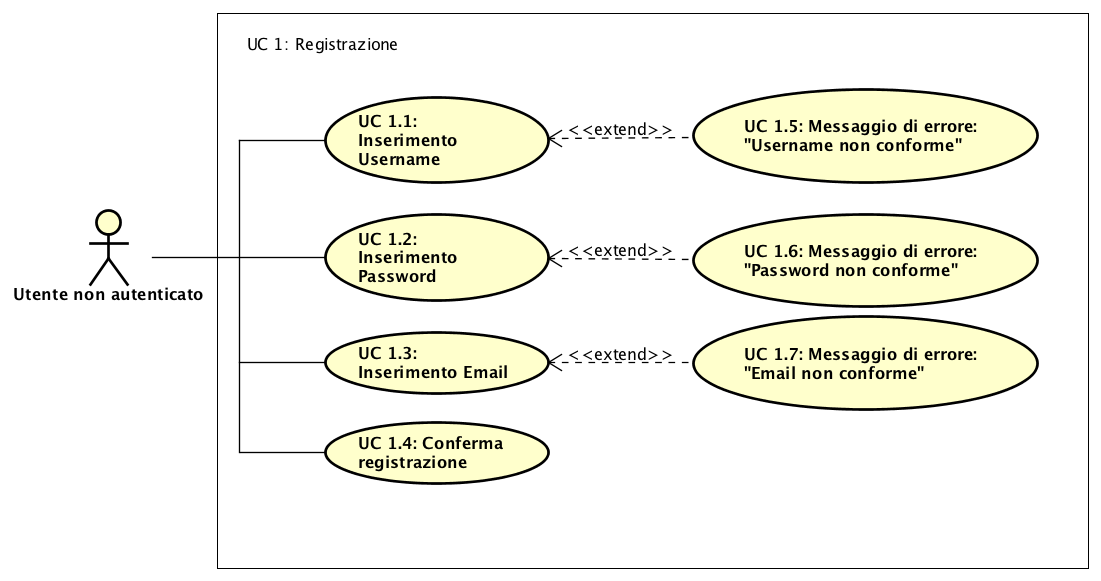
\includegraphics[scale=0.8]{../../Casi D'uso/UC1.png}
		\caption{Scelta della modalità di registrazione}
	\end{figure}
	\begin{itemize}
		\item \textbf{Attori coinvolti:} Utente non autenticato, che vuole interagire con il sistema. \\
		\item \textbf{Scopo e descrizione:} L'utente inserisce l'username che desidera utilizzare, la password che desidera utilizzare e uno dei propri indirizzi mail per effettuare la registrazione. \\
		\item \textbf{Precondizione:} Il sistema richiede all'utente le informazioni necessarie per effettuare la registrazione. \\
		\item \textbf{Postcondizione:} Il sistema elabora i dati inseriti dall'utente e, nel caso la registrazione avvenga con successo, gli concede la possibilità di accedere al sistema. In caso contrario viene visualizzato un messaggio d'errore e viene indicato dove è stato commesso, per l'appunto, l'errore. \\
	\end{itemize}
\subsection{UC 2: Autenticazione}
	\begin{figure}[h]
		\centering
		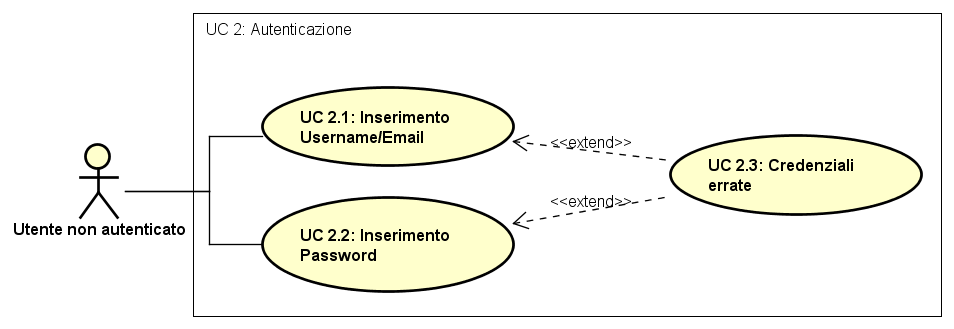
\includegraphics[scale=0.8]{../../Casi D'uso/UC2.png}
		\caption{Scelta della modalità di autenticazione}
	\end{figure}
	\begin{itemize}
		\item \textbf{Attori coinvolti:} Utente non autenticato, che vuole interagire con il sistema. \\
		\item \textbf{Scopo e descrizione:} L'utente inserisce il proprio username e la propria password per effettuare l'autenticazione. In caso di password dimenticata è possibile chiedere assistenza. \\
		\item \textbf{Precondizione:} L'utente decide di autenticarsi in maniera standard e il sistema richiede quindi l'inserimento delle informazioni necessarie per permettere l'operazione. \\
		\item \textbf{Postcondizione:} Il sistema elabora i dati forniti dall'utente e concede la possibilità di usufruire delle proprie funzionalità, se l'autenticazione avviene con successo. In caso contrario viene visualizzato un messaggio di autenticazione fallita e viene invitato l'utente a controllare i dati inseriti. \\
	\end{itemize}
